\documentclass[../ClassicThesis.tex]{subfiles}
\begin{document}
%************************************************
\chapter{Adjacency Plategraph / Klara}\label{ch:graph}
%************************************************

% Use active Voice (we do….)
% Ein Gedanke pro Paragraph
% Terminologie anpassen über alle Arbeiten hinweg (was ist eine Plate für alle…)
% Jeder sollte eine kleine Related Work section haben
% Erklärungen zu warum dieser Algorithmus genutzt wurde und nicht ein anderer + limitations des gewählten Algorithmus
% Hübsche Bildchen zum anschaulichen Erklären!! (ebenfalls konsistent halten: gleich geformte labels etc.)
% FROM SOLUTION TO PROBLEM /DISCUSSION
% EXPLAIN ALL VARIABLES ETC.!!!

% 1. Was macht es inhaltlich
% 2. Was kann/tut der Graph überhaupt?


% \paragraph{Why is this part necessary?}
On the basis of the graph we can create connectors for plates in a later step ( \ref{ch:joints}). Depending on angles and neighborhood relationships an adequate connector type can be chosen.
% for what? to figure out joint connections?

% \paragraph{What is being achieved in this Chapter?}
In this step we analyse the spatial arrangement of plate objects in 3D-space to create a graph structure which tracks the adjacency. The plates to be analysed are found in the previous step \ref{ch:plates}. Two or more plates are adjacent to another when at least one side touches or overlaps with another plate. In addition, the angles in between the plates are measured. 


% WHAT IS WITH THE 3D SNIPPETS??? DO THEY STILL EXIST?

% \paragraph{Chosen Graph Class Structure}
The graph always holds a list of all found plates and their neighbors. A plate is just one possible object to be listed. Other graph nodes can be left over 3D snippets which will have to be handled when all plates have been correctly connected.\\
For iterating over the graph we traverse all edges of the graph which also hold the important neighborhood parameters such as angle and the line at which nodes intersect.\\\* \\
\hspace*{-1.8cm}
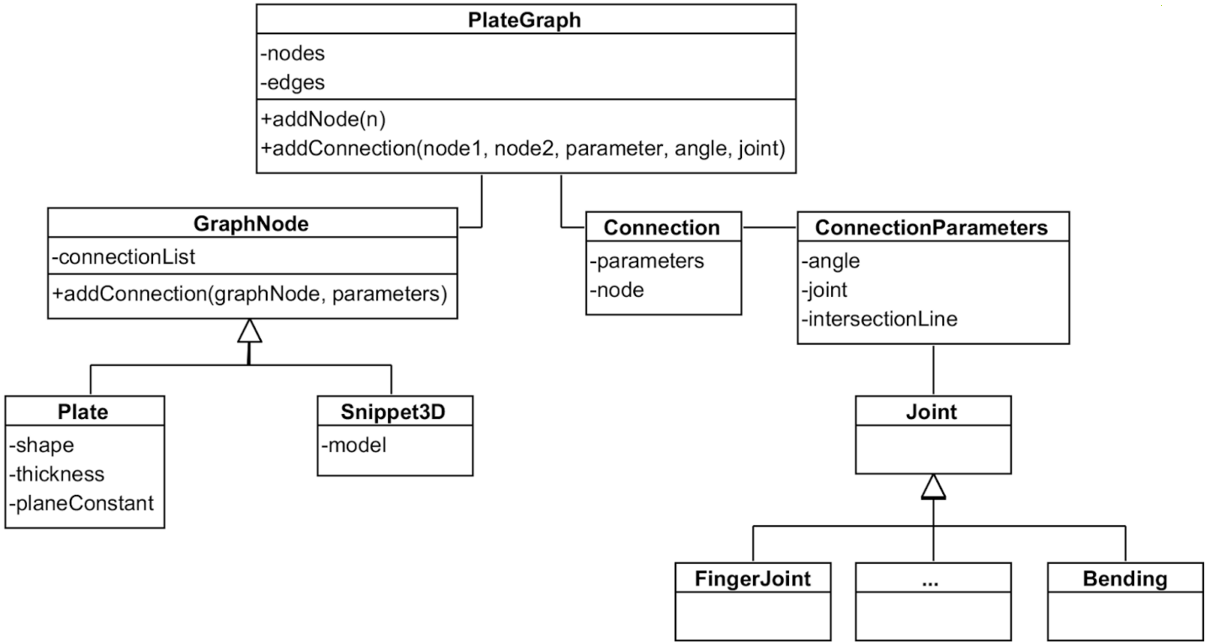
\includegraphics[width=1.3\columnwidth]{Images/GraphStructure.png}


\section{Analysing spatial arrangement}
% \subparagraph{requirements for running the algorithm}
% unnecessary??
As a prerequisite the step \ref{ch:plates} needs to find inherent or create extruded plates first. Afterwards the plane-plane intersections of all combinations of both sides of the plates are computed which results in up to four intersection lines. In preparation for the joint generation step \ref{ch:joints} we truncate the inner intersection lines which would otherwise overlap with adjacent plate intersections.

\subsection{Finding intersections}
% \subparagraph{concrete explanation, functions used/example code etc.}
When two planes intersect there is an intersection line. Since we work with plates which equal 2 parallel planes we expect to find up to 4 intersection lines.\\
Firstly, we retrieve the direction vector(\emph{dir}) of any intersection line between two plates by calculating the cross vector of both normals.\\
% TODO: include citation
In order to retrieve all possible intersection lines of two plates we calculate four possible plane-plane intersections \cite{planePlaneIntersection} of 
\begin{itemize}
\item the two main sides of the plates
\item the two parallel sides of the plates
\item one main and one parallel side 
\item and the other way around
\end{itemize}
\*\\
First, a possible position vector has to be found which lies on both planes.
\\\*\\
\emph{Plane constants:} $d_1, d_2$\\
\emph{Normals:} $n_1, n_2$
$$ p = \frac{d_1 * n_{2}^{2} - d_2 * (n_1 * n_2)}{n_{1}^{2} * n_{2}^{2} - (n_1 * n_2)^{2}} * n_1 + \frac{d_2*n_1^2 - d_1*(n_1 * n_2)}{n_1^2 * n_2^2 - (n_1 * n_2)^2} * n_2 $$

On the basis of a position vector an intersection line can be computed.
% TODO: make this nicer
$$ line = p*x + dir$$

Now that all lines are found we have to test if the lines actually go through both plates. In addition, this step retrieves the exact start and end points of the line segment that defines the intersection of both plates.\\
In order to find the boundaries of the lines we calculate the intersections of the lines with all boundary edges of the plates.\\
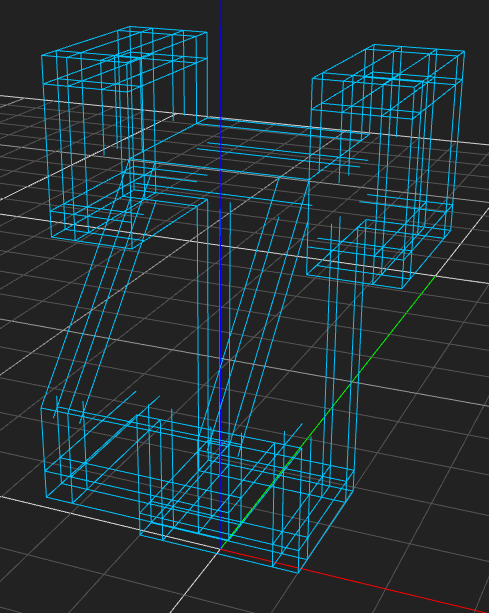
\includegraphics[width=.5\columnwidth]{Images/HeadAllBoundaries.png}

\subsection{Determine angles between plates}
In order to generate nicely fitting joints in the following step and for grouping plates the angles are necessary.\\
Firstly, we determine the angle between the according planes.\\
plane normals: u, v\\
angle between planes: $\theta$
$$ cos(\theta) = \frac{u \cdot v}{|u| * |v|}$$
But we are not talking about infinitely large planes instead we want the angle which is enclosed by the finitely large plates. Therefore we need to adjust the angle in some cases dependent on the direction in which the normals are pointing.
% figure which shows when angle is right, but also one case when it is not right
\begin{figure}[h]

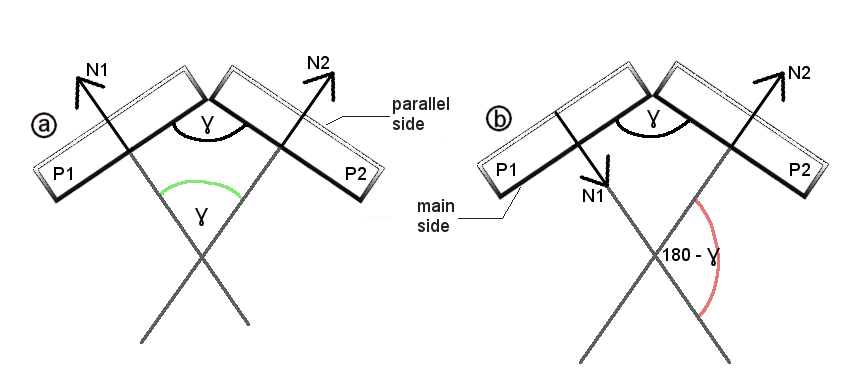
\includegraphics[width= 1\columnwidth]{Images/anglesExamplesSmall.png}
\caption{(a) The angle between the plates' normals correspond with the angle $\gamma$ between the plates. (b) The angle between the plates' normals is in this case an adjacent angle to the requested angle $\gamma$.}
\end{figure}

In order to find out in which cases the angle has to be adjusted we check for two properties.\\
Firstly, there is the question which of the sides of the plates intersect. A plate is defined by a 2D-shape which is called main side. The other side which exists due to a specified thickness of the plate is called parallel side.\\
Additionally, we look at the direction of the normals. The direction is positive when it is directed from the main to the parallel side and negative otherwise.\\
For an angle to be in need to be adjusted the following conditions need to be satisfied.
\begin{itemize}
    \item The two plates touch with the same type of side 
    \item[] AND
    \item Their directions are both positive OR both negative
\end{itemize}



\subsection{Truncating intersection lines}
Now that all lines are known we need to shorten the lines so that no other lines overlap with it. If this step is missing then the following step for creating joints will run in to problems that the joints overlap each other.\\
If we now have a look at only the inner intersections of plates in a model we can identify the overlaps.
\begin{figure}[t]
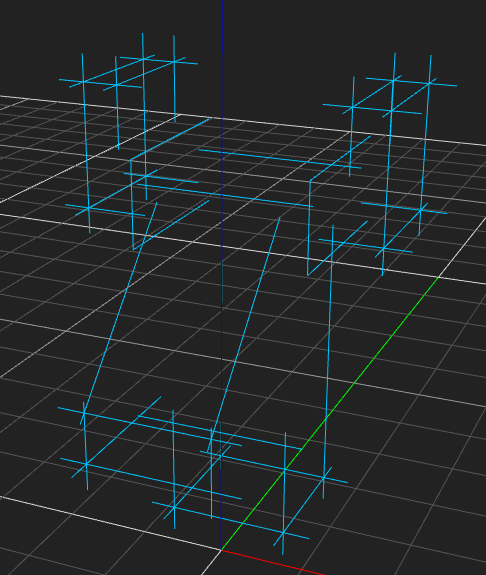
\includegraphics[width=.5\columnwidth]{Images/HeadInnerBoundaries.png}
\caption{The inner boundaries of the plates overlap. In the next step when joints will be created they are only supposed to be on the inner part of the line. Therefore the lines have to be truncated.}
\end{figure}
\*\\
\begin{algorithm}[H]
	\DontPrintSemicolon
	\KwData{lines}
	\KwResult{truncated lines}
	initialize variables here\;
    \For{line$\_$pair in lines}{
    	line1 = line$\_$pair[0]\;
        line2 = line$\_$pair[1]\;
        point = lineLineIntersection(line1, line2)\;
        \If{isPointOnLine(point, line1) and isPointOnLine(point, line2)}
        {
       		\tcp{linesegments actually cross}
       		startSegmentLine1 = new Line(point, line1.start)\;
            endSegmentLine1 = new Line(point, line1.end)\;
            startSegmentLine2 = new Line(point, line2.start)\;
            endSegmentLine2 = new Line(point, line2.end)\;
            \tcp{the shorter part of each line is discarded}
			\eIf{startSegmentLine1.distance() $>$ endSegmentLine1.distance()}{
				\eIf{startSegmentLine2.distance() $>$ endSegmentLine2.distance()}{
				return \{
                    	endSegmentLine1\;
                        endSegmentLine2
                    \}
				}{
                    return \{
                    	endSegmentLine1\;
                        startSegmentLine2
                    \}
				}
			}{
			return \{
                	startSegmentLine1\;
                    startSegmentLine2
                \}
			}	      
        }
    }
   	\caption{Truncate lines}
\end{algorithm}



\section{Alternative Solutions}
\subsection{Dustin: how he did it}
\subsection{Dustins wrong/not specified angles}
he didnt actually specify how he calculated the angles...
\subsection{Down sides}
\subsection{Whats better now?}

\section{How we got there}
\subsection{Floating Point inaccuracy}
\subsection{Bruteforce finding lines}
\subsection{different line intersection algorithms}

\section{Future work}
- find out if model is assemblable in the end
- rejoining broken up plates (t-connection)




% Dummy algorithm:\\
% \begin{algorithm}[H]
% 	\DontPrintSemicolon
% 	\KwData{input Data}
% 	\KwResult{result Data}
% 	initialize variables here\;
%    \caption{Name of Algorithm}

% \end{algorithm}



% \begin{algorithm}[H]
% \DontPrintSemicolon
% 	\KwData{this text}
% 	\KwResult{how to write algorithm with \LaTeX2e }
% 	initialization\;
% 	\While{not at end of this document}{
% 	read current\;
% 	\eIf{understand}{
% 	go to next section\;
% 	current section becomes this one\;
% 	}{
% 	go back to the beginning of current section\;
% 	}
%      \For{all I know}{
%      look at this link to learn more about \LaTeX2e:\;
%      http://ctan.space-pro.be/tex-archive/macros/latex/contrib/algorithm2e/doc/algorithm2e.pdf\;
%      }
% 	}
%    \caption{How to write algorithms}

% \end{algorithm}






\end{document}